\documentclass[a4paper, 12pt]{article}

\usepackage[portuges]{babel}
\usepackage[utf8]{inputenc}
\usepackage{amsmath}
\usepackage{indentfirst}
\usepackage{blindtext}
\usepackage{graphicx}
\usepackage[hidelinks]{hyperref}
\usepackage{gensymb}
\usepackage{pgfplots}

\author{Igor Abreu da Silva}

\title{Trabalho Final de Sistemas Lineares I}

\begin{document}

    \begin{titlepage}
        \begin{center}
            \huge{Universidade Federal do Rio de Janeiro}
            \vspace{95pt}

            \large{Lista I - Sistemas Lineares I}
            \vspace{160pt}
        \end{center}

        \begin{flushleft}
            \begin{tabbing}
                Alunos\qquad\qquad\= Igor Abreu da Silva\\
                DRE\> 112053874 \\
                Curso\> Engenharia Eletrônica \\
                Turma\> 2016/2 \\
                Professor\> Natanael Nunes de Moura Junior \\

            \end{tabbing}

        \end{flushleft}

        \begin{center}
            \vspace{\fill}
            Rio de Janeiro, 16 de Setembro de 2016
        \end{center}
    \end{titlepage}

    \newpage
    \tableofcontents
    \listoffigures
    \thispagestyle{empty}
    \newpage
    \pagenumbering{arabic}

    \section{Quest\~{a}o 1 - Conhecimentos Básicos}
        \subsection{Item a}
            \begin{figure}[!ht]
                \centering
                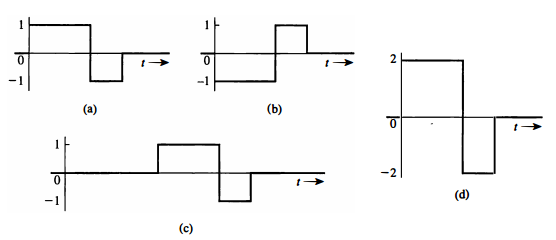
\includegraphics{img/Figura1.PNG}
                \caption{Sinais utilizados no Item A}
            \end{figure}
            Analisando os resultados, percebe-se que a inversão ou o deslocamento não alteram a energia do sinal, entretanto, a multiplicação por um fator k altera o sinal em $k^{2}$.
            \subsubsection{Sinal (a)}
            $\int_{0}^{2} 1^{2}dx + \int_{2}^{3} -1^{2}dx \Rightarrow  \int_{0}^{2}dx + \int_{2}^{3}dx = 3$
            \subsubsection{Sinal (b)}
            $\int_{0}^{2} -1^{2}dx + \int_{2}^{3} 1^{2}dx \Rightarrow  \int_{0}^{2}dx + \int_{2}^{3}dx = 3$
            \subsubsection{Sinal (c)}
            $\int_{3}^{5} 1^{2}dx + \int_{5}^{6} -1^{2}dx \Rightarrow  \int_{3}^{5}dx + \int_{5}^{5}dx = 3$
            \subsubsection{Sinal (d)}
            $\int_{0}^{2} 2^{2}dx + \int_{2}^{3} -2^{2}dx \Rightarrow  \int_{0}^{2}4dx + \int_{2}^{3}4dx = 12$
            \newpage
        \subsection{Item b}
            \begin{figure}[!ht]
                \centering
                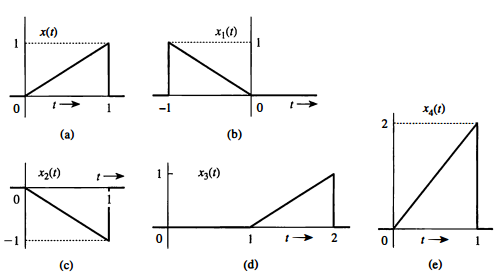
\includegraphics{img/Figura2.PNG}
                \caption{Sinais utilizados no Item B}
            \end{figure}
            Repete-se o que ocorre no Item(a)
            \subsubsection{Sinal (a)}
            $\int_{0}^{1} x^{2}dx  = \frac{1}{3}$
            \subsubsection{Sinal (b)}
            $\int_{-1}^{0} (-x)^{2}dx  = \frac{1}{3}$
            \subsubsection{Sinal (c)}
            $\int_{0}^{1} (-x)^{2}dx  = \frac{1}{3}$
            \subsubsection{Sinal (d)}
            $\int_{1}^{2} (x-1)^{2}dx  \Rightarrow \int_{1}^{2} (x^{2}-2x+1)dx = \frac{8}{3} - \frac{1}{3} - 4 +1 + 2 -1 = \frac{1}{3}$
            \subsubsection{Sinal (e)}
            $\int_{0}^{1} (2x)^{2}dx  = \frac{4}{3}$
        \subsection{Item c}
            \begin{figure}[!ht]
                \centering
                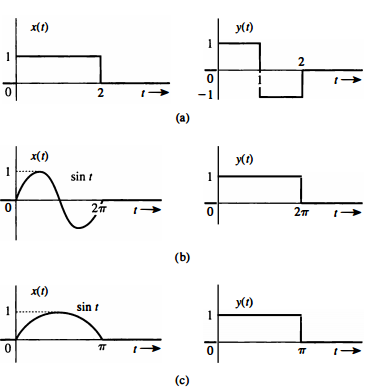
\includegraphics{img/Figura3.PNG}
                \caption{Sinais utilizados no Item C}
            \end{figure}
            Percebe-se que nos Sinais "a" e "b" a energia de x+y é igual a energia de x e y somadas, assim com, x-y é a energia de "a" e "b" subtraída, entretanto, não podemos assumir isso como verdade pois nos Sinais "c" não existe tal relação.
            \subsubsection{Sinais (a)}
            \[E_{x} = \int_{0}^{2} 1^{2}dx = 2 \]
            \[E_{y} = \int_{0}^{1} 1^{2}dx + \int_{1}^{2} -1^{2}dx \Rightarrow 1 + 1 = 2 \]
            \[E_{x+y} = \int_{0}^{1} 2^{2}dx = 4 \]
            \[E_{x-y} = \int_{1}^{2} -2^{2}dx = 4 \]
            \subsubsection{Sinais (b)}
            \[E_{x} = \int_{0}^{2\pi} sin^{2}(x)dx \Rightarrow \int_{0}^{2\pi} \frac{1-cos(2x)}{2} \Rightarrow  \frac{1}{2}\int_{0}^{2\pi} 1dx - \frac{1}{2}\int_{0}^{2\pi} cos(2x)dx = \pi + 0 = \pi\]
            \[E_{y} = \int_{0}^{2\pi} 1^{2}dx  = 2\pi \]
            \[E_{x+y} = \int_{0}^{2\pi} (sin(x) +1)^{2}dx \Rightarrow \int_{0}^{2\pi} \frac{1-cos(2x)}{2} + 2sen(x) + 1\Rightarrow\]\[ \frac{1}{2}\int_{0}^{2\pi} 1dx - \frac{1}{2}\int_{0}^{2\pi} cos(2x)dx + 2\int_{0}^{2\pi} sin(x)dx + \int_{0}^{2\pi} 1dx= \pi + 0 + 0 + 2\pi = 3\pi\]
            \[E_{x-y} = \int_{0}^{2\pi} (sin(x) -1)^{2}dx \Rightarrow \int_{0}^{2\pi} \frac{1-cos(2x)}{2} - 2sen(x) + 1\Rightarrow\]\[ \frac{1}{2}\int_{0}^{2\pi} 1dx - \frac{1}{2}\int_{0}^{2\pi} cos(2x)dx - 2\int_{0}^{2\pi} sin(x)dx + \int_{0}^{2\pi} 1dx= \pi + 0 + 0 + 2\pi = 3\pi\]
            \subsubsection{Sinais (c)}
            \[E_{x} = \int_{0}^{\pi} sin^{2}(x)dx \Rightarrow \int_{0}^{\pi} \frac{1-cos(2x)}{2} = \frac{\pi}{2} + 0 = \frac{\pi}{2} \]
            \[E_{y} = \int_{0}^{\pi} 1^{2}dx = \pi\]
            \[E_{x+y} = \int_{0}^{\pi} (sin + 1)^{2}dx \Rightarrow \int_{0}^{\pi} \frac{1-cos(2x)dx}{2} + \int_{0}^{\pi}2sin(x) + \int_{0}^{\pi}dx = \frac{\pi}{2} + 4 + \pi = \frac{3\pi}{2} + 4\]
            \[E_{x-y} = \int_{0}^{\pi} (sin - 1)^{2}dx \Rightarrow \int_{0}^{\pi} \frac{1-cos(2x)dx}{2} + \int_{0}^{\pi}-2sin(x) + \int_{0}^{\pi}dx = \frac{\pi}{2} - 4 + \pi = \frac{3\pi}{2} - 4\]
            \newpage
        \subsection{Item d}
            \begin{figure}[!ht]
                \centering
                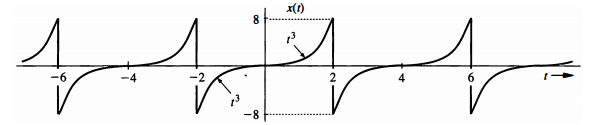
\includegraphics{img/Figura4.PNG}
                \caption{Sinais utilizados no Item D}
            \end{figure}
            \[P(x) = \frac{1}{4} \int_{-2}^{2} (x^{3})^{2}dx = \frac{64}{7}\]
            Percebe-se, que a inversão do sinal não altera a potência, entretanto a multiplicação por um escalar C, altera a potência em $C^{2}$, um comportamento igual ao já provado no calculo de energia.
            \subsubsection{Sinais (a)}
            \[P(-x) = \frac{1}{4} \int_{-2}^{2} (-x^{3})^{2}dx = \frac{64}{7}\]
            \subsubsection{Sinais (b)}
            \[P(2x) = \frac{1}{4} \int_{-2}^{2} (2x^{3})^{2}dx = \frac{256}{7}\]
            \subsubsection{Sinais (c)}
            \[P(Cx) = \frac{1}{4} \int_{-2}^{2} (Cx^{3})^{2}dx = \frac{64C^{2}}{7}\]
            \newpage
        \subsection{Item e}
            \subsubsection{Sinais (a)}
                \begin{tikzpicture}
                \begin{axis}[%
                ,xlabel=$t$
                ,ylabel=$u(t)$
                ,axis x line = bottom,axis y line = left
                ,ytick={1,2}
                ,ymax=2.5 % or enlarge y limits=upper
                ]
                \addplot+[const plot, no marks, thick] coordinates {(0,0) (1,0) (2,0) (3,0) (4,0) (5,1) (6,1) (7,1)(7,0) (8,0)} node[above,pos=.57,black]{};
                \end{axis}
                \end{tikzpicture}
            \subsubsection{Sinais (b)}
                \begin{tikzpicture}
                \begin{axis}[%
                ,xlabel=$t$
                ,ylabel=$u(t)$
                ,axis x line = bottom,axis y line = left
                ,ytick={1,2}
                ,ymax=2.5 % or enlarge y limits=upper
                ]
                \addplot+[const plot, no marks, thick] coordinates {(0,0) (1,0) (2,0) (3,0) (4,0) (5,1) (6,1) (7,2)(8,2) } node[above,pos=.57,black]{};
                \end{axis}
                \end{tikzpicture}
            \subsubsection{Sinais (c)}
                \begin{tikzpicture}
                \begin{axis}[%
                ,xlabel=$t$
                ,ylabel=$u(t)$
                ,axis x line = bottom,axis y line = left
                ,ytick={1,2,3,4}
                ,ymax=4 % or enlarge y limits=upper
                ]
                \addplot+[const plot, no marks, thick] coordinates {(0,0) (1,0) (1,1)} {};
                \addplot[domain=1:2,blue]{x*x};
                \addplot+[const plot, no marks, thick,blue] coordinates {(2,4) (2,0) (3,0)} {};
                \end{axis}
                \end{tikzpicture}
            \subsubsection{Sinais (d)}
                \begin{tikzpicture}
                \begin{axis}[%
                ,xlabel=$t$
                ,ylabel=$u(t)$
                ,axis x line = bottom,axis y line = left
                ,ytick={-1,-2,0,1,2}
                ,ymax=2 % or enlarge y limits=upper
                ,ymin=-2
                ]
                \addplot+[const plot, no marks, thick] coordinates {(0,0) (1,0) (2,0) (2,-2)} {};
                \addplot[domain=2:4,blue]{(x-4)};
                \addplot+[const plot, no marks, thick,blue] coordinates {(4,0) (5,0)} {};
                \end{axis}
                \end{tikzpicture}
        \subsection{Item f}
            \subsubsection{Sinais (a)}
            Impulso unitário em sin(0) = 0
            \subsubsection{Sinais (b)}
            $\frac{2}{9}\delta(\omega)$
            \subsubsection{Sinais (c)}
            $1(cos(-60)) = \frac{1}{2}\delta(t)$
            \subsubsection{Sinais (d)}
            $\frac{sin(\frac{-\pi}{2})}{(1)^{2}+4} = \frac{-1}{5}\delta(1-t)$
            \subsubsection{Sinais (e)}
            Substituindo-se $\omega + 3$ em $\omega$, teremos: $\frac{1}{-3j + 2}\delta(\omega+3)$
            \subsubsection{Sinais (f)}
            Usando L'hopital em $\frac{sin(k\omega)}{\omega}$, temos: $kcos(k\omega)$ que com $\omega = 0$ temos: $k\delta(\omega)$
        \subsection{Item g}
            \subsubsection{Sinais (a)}
            Como o impulso é localizado em $\tau = t$, nesse caso temos $x(\tau) = x(t)$ logo, essa integral é igual a x(t).
            \subsubsection{Sinais (b)}
            Em $\delta(\tau)$ o impulso é realizado em $\tau$ = 0, sendo $\tau = 0$, temos o resultado = x(t).
            \subsubsection{Sinais (c)}
            O impulso ocorre em t=0 nesta caso temos $e^{0} = 1$.
            \subsubsection{Sinais (d)}
            O impuso ocorre em t = 0, logo $sin(3\pi) = 0$.
            \subsubsection{Sinais (e)}
            O impulso ocorre em t = -3, logo o resultado sera $e^{3}$.
            \subsubsection{Sinais (f)}
            O impulso ocorre em t = 1, logo o resultado sera $1^{3} + 4 = 5$.
            \subsubsection{Sinais (g)}
            O impulso ocorre em t = 3, logo o resultado sera $x(2-3) = x(-1)$.
            \subsubsection{Sinais (h)}
            O impulso ocorre quando t = 3, logo o resultado sera $e^{3-1}cos(-\pi) = -e^{2}$.
        \subsection{Item h}
            \subsubsection{Sinais (a)}
            $cos(\omega t) = \frac{e^{\alpha t + j\omega t} + e^{\alpha t - j\omega t}}{2}$, $\alpha = 0$ pois e função é uma senoide e $\omega = 3$, sabendo-se que $s = \alpha + j\omega$ temos: $s_{1} = j3$ e $ s_{2} = -j3 $
            \subsubsection{Sinais (b)}
            Nesse caso, temos $\alpha = -3$ e $\omega = 3$, logo $s_{1} = -3 + j3$ e $s_{2} = -3 - j3$
            \subsubsection{Sinais (c)}
            Nesse caso, temos $\alpha = 2$ e $\omega = 3$, logo $s_{1} = 2 + j3$ e $s_{2} = 2 - j3$
            \subsubsection{Sinais (d)}
            Nesse caso, temos $\alpha = -2$ e $\omega = 0$, logo $s = -2$
            \subsubsection{Sinais (e)}
            Nesse caso, temos $\alpha = 2$ e $\omega = 0$, logo $s = 2$
            \subsubsection{Sinais (f)}
            Nesse caso, temos $\alpha = 0$ e $\omega = 0$, logo $ke^{0}$ tendo k = 5
        \subsection{Item i}
            \subsubsection{Sinais (a)}
            Pode se dizer que $x(t)_{par} = \frac{x(t)}{2} + \frac{x(-t)}{2}$ e $x(t)_{impar} = \frac{x(t)}{2} + \frac{-x(-t)}{2}$, logo $\int_{-\infty}^{\infty} [\frac{x(t)}{2} + \frac{x(-t)}{2}][\frac{x(t)}{2} + \frac{-x(-t)}{2}] = \int_{-\infty}^{\infty} (\frac{x(t)}{2})^{2} - (\frac{x(-t)}{2})^{2} $ como o modulo de x(t) é igual ao modulo de x(-t) essa integral resultara em 0.
            \subsubsection{Sinais (b)}
            Pode se dizer que $x(t)_{par} = \frac{x(t)}{2} + \frac{x(-t)}{2}$, logo $\int_{-\infty}^{\infty} \frac{x(t)}{2} + \frac{x(-t)}{2}$ como x(t) = x(-t) $\int_{-\infty}^{\infty} x(t)$.
        \subsection{Item j}
            \subsubsection{Sinais (a)}
            \[x_{1}(t)  \Rightarrow ay_{1}^{'}(t) + 2ay_{1}(t) = ax_{1}^{2}(t)\]
            \[x_{2}(t)  \Rightarrow by_{2}^{'}(t) + 2by_{2}(t) = bx_{2}^{2}(t)\]
            \[x_{3}(t)  \Rightarrow y_{3}^{'}(t) + 2y_{3}(t) = x_{3}^{2}(t) \Rightarrow (ax_{1}(t) + bx_{2}(t))^{2} \Rightarrow a^{2}x_{1}^{2}(t) + 2abx_{1}(t)x_{2}(t) + b^{2}x_{2}^{2}(t)\]
            $a^{2}x_{1}^{2}(t) + 2abx_{1}(t)x_{2}(t) + b^{2}x_{2}^{2}(t)$ não é igual à  $ax_{1}^{2}(t) + bx_{2}^{2}(t)$, logo o sistema não é linear.
            \subsubsection{Sinais (b)}
            \[x_{1}(t)  \Rightarrow ay_{1}^{'}(t) + 3aty_{1}(t) = ax_{1}t^{2}(t)\]
            \[x_{2}(t)  \Rightarrow by_{2}^{'}(t) + 3bty_{2}(t) = bx_{2}t^{2}(t)\]        
			\[x_{3}(t)  \Rightarrow y_{3}^{'}(t) + 3ty_{3}(t) = x_{3}t^{2}(t) \Rightarrow (ax_{1}(t) + bx_{2}(t))t^{2} \]   
			$(ax_{1}(t) + bx_{2}(t))t^{2}$ é igual à $ax_{1}t^{2}(t) + bx_{2}t^{2}(t)$, logo o sistema é linear
            \subsubsection{Sinais (c)}
            \[x_{1}(t)  \Rightarrow a3y_{1}(t) + 2 = ax_{1}(t)\]
            \[x_{2}(t)  \Rightarrow b3y_{2}(t) + 2 = bx_{2}(t)\]   
			\[x_{3}(t)  \Rightarrow y_{3}(t) + 2 = x_{3}(t) \Rightarrow [a3y_{1}(t) + b3y_{2}(t)] +2 =  [ax_{1}(t) + bx_{2}(t)]\] isso é diferente de $a3y_{1}(t) + b3y_{2}(t) + 4 = [ax_{1}(t) + bx_{2}(t)]$ logo não é linear              
                        
            \subsubsection{Sinais (d)}
            \[x_{1}(t)  \Rightarrow ay_{1}^{'}(t) + ay_{1}^{2}(t) = ax_{1}(t)\]
            \[x_{2}(t)  \Rightarrow by_{2}^{'}(t) + by_{2}^{2}(t) = bx_{2}(t)\]    
			\[x_{3}(t)  \Rightarrow y_{3}^{'}(t) + y_{3}^{2}(t) = x_{3}(t) \Rightarrow [ay_{1}^{'}(t) + by_{2}^{'}(t)] + [ay_{1}(t) + by_{2}(t)]^{2} =  [ax_{1}(t) + bx_{2}(t)]\], o valor quadrático gerará um termo que fara com que esse sistema não seja linear.                      
            \subsubsection{Sinais (e)}
            \[ x_{1}(t) \Rightarrow ay_{1}^{'2}(t) + 2ay_{1}(t)  = ax_{1}(t)\]
            \[ x_{2}(t) \Rightarrow by_{2}^{'2}(t) + 2by_{2}(t)  = bx_{2}(t)\]      
			\[ x_{3}(t) \Rightarrow y_{3}^{'2}(t) + 2y_{3}(t) = x_{3}(t) \Rightarrow [ay_{1}^{'}(t) + by_{2}^{'}(t)]^{2} + 2[ay_{1}(t) + by_{2}(t)] =  [ax_{1}(t) + bx_{2}(t)]\] o valor quadrático gerará um termo que fara com que esse sistema não seja linear.                                        
            \subsubsection{Sinais (f)}
            \[ x_{1}(t) \Rightarrow ay_{1}^{'}(t) + asin(t)y_{1}(t)  = ax_{1}^{'}(t) + 2ax_{1}(t)\]
            \[ x_{2}(t) \Rightarrow by_{2}^{'}(t) + bsin(t)y_{2}(t)  = bx_{2}^{'}(t) + 2bx_{2}(t)\]             
			\[ x_{3}(t) \Rightarrow y_{3}^{'}(t) + sin(t)y_{3}(t) =  x_{3}^{'}(t) + 2x_{3}(t) \Rightarrow\] 
			\[[ay_{1}^{'}(t) + by_{2}^{'}(t)] + sin(t)[ay_{1}(t) + by_{2}(t)] = [ax_{1}^{'} + bx_{2}^{'}] + 2[ax_{1}(t) + bx_{2}(t)]\]. O sistema é linear.            
            \subsubsection{Sinais (g)}
            \[ x_{1}(t) \Rightarrow ay_{1}^{'}(t) + 2ay_{1}(t) = ax_{1}(t)x_{1}^{'}(t)\]
            \[ x_{2}(t) \Rightarrow by_{2}^{'}(t) + 2by_{2}(t) = bx_{2}(t)x_{2}^{'}(t)\]  
			\[ x_{3}(t) \Rightarrow y_{3}^{'}(t) + 2y_{3}(t) = x_{3}(t)x_{3}^{'}(t) \Rightarrow [ay_{1}^{'}(t) + by_{2}^{'}(t)] + 2[ay_{1}(t) + 2by_{2}(t)] = \]             
			\[[ax_{1}(t) + bx_{2}(t)][x_{1}^{'}(t)+x_{2}^{'}(t)]\]. A multiplicação cruzada do ultimo termo gerará um valor tal que o sistema não será linear.
            \subsubsection{Sinais (h)}
            \[ x_{1}(t) \Rightarrow ay_{1}(t) = \int_{-\infty}^{t}x_{1}(\tau)d\tau\]
            \[ x_{2}(t) \Rightarrow by_{2}(t) = \int_{-\infty}^{t}x_{2}(\tau)d\tau\]        
            \[ x_{3}(t) \Rightarrow y_{3}(t) = \int_{-\infty}^{t}x_{3}(\tau)d\tau \Rightarrow [ay_{1}(t) + by_{2}(t) ] =  \int_{-\infty}^{t}[x_{1}(\tau) + x_{2}(\tau)]d\tau\ \]. O Sistema é linear.               
        \subsection{Item k}
            \subsubsection{Sinais (a)}
            $y_{1}(t) = x_{1}(t-2) $ considerando $x_{2}(t) = x_{1}(t-2-t_{0})$, temos: $y_{2}(t) = x_{2}(t) = x_{1}(t-2-t_{0})$. $y_{1}(t-t_{0}) =  x_{1}(t-2-t_{0})$, logo pode-se concluir que $y_{2}(t) = y_{1}(t-t_{0})$ com isso o sistema é invariante no tempo.
            
            \subsubsection{Sinais (b)}
            $y_{1}(t) = x_{1}(-t)$, considerando $x_{2}(t) = x_{1}(-t-t_{0})$, temos: $y_{2}(t) = x_{2}(-t) = x_{1}(-t-t_{0})$, logo $y_{1}(-t-t_{0}) = x_{1}(t+t_{0})$. O sistema é variante com o tempo.
            \subsubsection{Sinais (c)}
            $y_{1}(t) = x_{1}(at)$, considerando $x_{2}(at) = x_{1}(at-t_{0})$, temos: $y_{2}(t) = x_{2}(at) = x_{1}(at-t_{0})$, logo $y_{1}(at-t_{0}) = x_{1}(a(at+t_{0}))$. O sistema é variante com o tempo.            
            \subsubsection{Sinais (d)}
            $y_{1}(t) = tx_{1}(t-2) $ considerando $x_{2}(t) = x_{1}(t-2-t_{0})$, temos: $y_{2}(t) = tx_{2}(t) = tx_{1}(t-2-t_{0})$. $y_{1}(t-t_{0}) =  (t-t_{0})x_{1}(t-2-t_{0})$, logo pode-se concluir que é variante no tempo.
            \subsubsection{Sinais (e)}
            $y_{1}(t) = \int_{-5}^{5}x_{1}(\tau)d\tau $ considerando $x_{2}(\tau) = x_{1}(\tau-t_{0})$, temos: $y_{2}(t) = \int_{-5}^{5}x_{2}(\tau)d\tau = \int_{-5}^{5}x_{1}(\tau-t_{0})d\tau$. $y_{1}(\tau-t_{0}) =  \int_{-5}^{5}x_{1}(\tau - t_{0})d\tau$, logo pode-se concluir que é invariante no tempo.            
            \subsubsection{Sinais (f)}
            $y_{1}(t) = x_{1}^{'2}(t) $ considerando $x_{2}(t) = x_{1}(t-t_{0})$, temos: $y_{2}(t) = x_{2}^{'2}(t) = x_{1}^{'2}(t-t_{0})$. $y_{1}(t-t_{0}) = x_{1}^{'2}(t-t_{0})$, logo pode-se concluir que é invariante no tempo.            
        \subsection{Item l}
        \[y_{1} = \frac{x^{2}_{1}(t)}{x_{1}^{'}(t)}\]
        \[y_{2} = \frac{x^{2}_{2}(t)}{x_{2}^{'}(t)}\]
        \[y_{3} = \frac{x^{2}_{3}(t)}{x_{3}^{'}(t)} \Rightarrow [y_{1} + y_{2}] = \frac{(x_{1}(t) + x_{2}(t))^{2} }{x_{1}^{'}(t) + x_{2}^{'}(t)}\] não é aditiva.
        \[ay_{1} = \frac{(ax_{1})^{2}(t)}{ax_{1}^{'}(t)} \Rightarrow y_{1} = a[\frac{(x_{1})^{2}(t)}{x_{1}^{'}(t)}] = ay_{1}\] é homogênea.
           
        \subsection{Item m}
            \subsubsection{Sinais (a)}
            \subsubsection{Sinais (b)}
            \subsubsection{Sinais (c)}
            \subsubsection{Sinais (d)}
            \subsubsection{Sinais (e)}
            \subsubsection{Sinais (f)}
        \subsection{Item n}
            \begin{figure}[!ht]
                \centering
                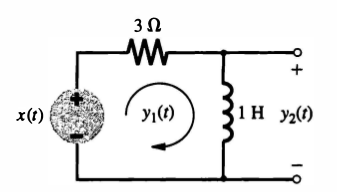
\includegraphics{img/Figura5.PNG}
                \caption{Circuito 1}
            \end{figure}
    \section{Quest\~{a}o 2 - Conhecimentos Básicos}
        \subsection{Item a}
            \subsubsection{Sinais (a)}
            \subsubsection{Sinais (b)}
            \subsubsection{Sinais (c)}
            \subsubsection{Sinais (d)}
            \subsubsection{Sinais (e)}
        \subsection{Item b}
            \subsubsection{Sinais (a)}
            \subsubsection{Sinais (b)}
            \subsubsection{Sinais (c)}
        \subsection{Item c}
            \subsubsection{Sinais (a)}
            \subsubsection{Sinais (b)}
            \subsubsection{Sinais (c)}
            \subsubsection{Sinais (d)}
        \subsection{Item d}
            \subsubsection{Sinais (a)}
            \subsubsection{Sinais (b)}
            \subsubsection{Sinais (c)}
            \subsubsection{Sinais (d)}
            \subsubsection{Sinais (e)}
        \subsection{Item e}
        \subsection{Item f}
        \subsection{Item g}
            \subsubsection{Sinais (a)}
            \subsubsection{Sinais (b)}
            \subsubsection{Sinais (c)}
            \subsubsection{Sinais (d)}
            \subsubsection{Sinais (e)}
            \subsubsection{Sinais (f)}
        \subsection{Item h}
            \subsubsection{Sinais (a)}
            \subsubsection{Sinais (b)}
            \subsubsection{Sinais (c)}
            \subsubsection{Sinais (d)}
            \subsubsection{Sinais (e)}
            \subsubsection{Sinais (f)}
            \subsubsection{Sinais (g)}
    \section{Quest\~{a}o 3 - Conhecimentos Básicos}
        \subsection{Item a}
        \subsection{Item b}
        \subsection{Item c}
        \subsection{Item d}
        \subsection{Item e}
    \section{Quest\~{a}o 4 - Conhecimentos Básicos}
        \subsection{Item a}
        \subsection{Item b}
        \subsection{Item c}
    \section{Quest\~{a}o 5 - Classificação de Sinais}
    \section{Quest\~{a}o 6 - Classificação de Sistemas}
        \subsection{Item a}
        \subsection{Item b}
        \subsection{Item c}
    \section{Quest\~{a}o 7 - Classificação de Sistemas}
        \subsection{Item a}
        \subsection{Item b}
    \section{Quest\~{a}o 8 - Energia e Potência de Sinais}
    \section{Quest\~{a}o 9 - Operação com Sinais}
        \subsection{Item a}
        \subsection{Item b}
        \subsection{Item c}
        \subsection{Item d}
    \section{Quest\~{a}o 10 - Operação com Sinais}
        \subsection{Item a}
        \subsection{Item b}
\end{document}